\usetikzlibrary {positioning}
\definecolor{red}{HTML}{8A3F3A}
\definecolor{yellow}{HTML}{E0BB3C}
\definecolor{blue}{HTML}{4569E0}
\definecolor{green}{HTML}{17E561}
\definecolor{other}{HTML}{6A939E}

% DTU Colors
\definecolor{dtu-corporate-red}{HTML}{990000}
\definecolor{dtu-white}{HTML}{ffffff}
\definecolor{dtu-black}{HTML}{000000}
\definecolor{dtu-blue}{HTML}{2F3EEA}
\definecolor{dtu-bright-green}{HTML}{1FD082}
\definecolor{dtu-navy-blue}{HTML}{030F4F}
\definecolor{dtu-yellow}{HTML}{F6D04D}
\definecolor{dtu-orange}{HTML}{FC7634}
\definecolor{dtu-pink}{HTML}{F7BBB1}
\definecolor{dtu-grey}{HTML}{DADADA}
\definecolor{dtu-red}{HTML}{E83F48}
\definecolor{dtu-green}{HTML}{008835}
\definecolor{dtu-purple}{HTML}{79238E}


\pgfkeys{
	/uncertaintyComplexity/.is family,
	/uncertaintyComplexity,
	show_useless_operation_research/.initial = false,
	show_simplistic_heuristics/.initial = false,
}

\newcommand{\drawUncertaintyComplexityValue}[1][]{
	\pgfkeys{\uncertaintyComplexity, #1}

	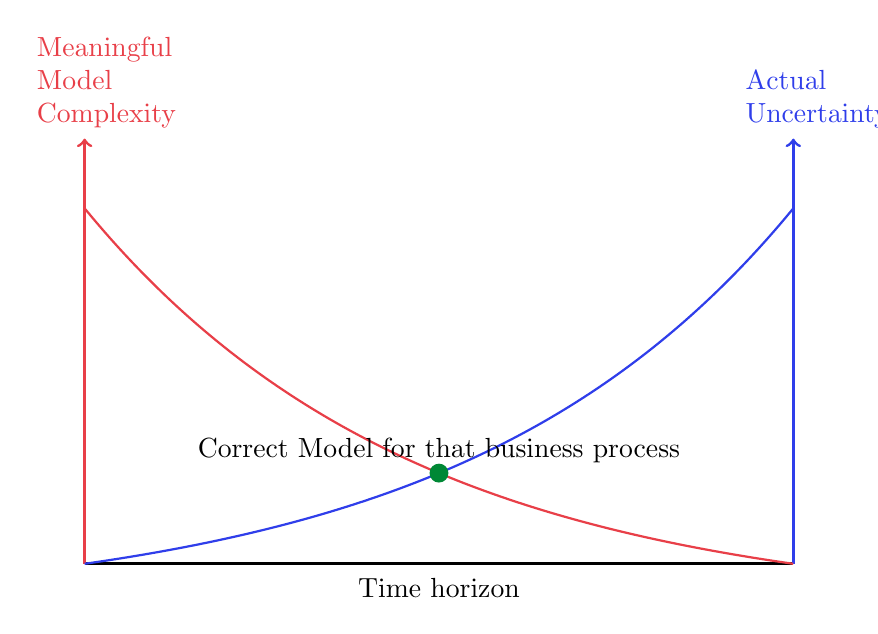
\begin{tikzpicture}[scale=0.6, line width=1.05][]

	\draw[-] (0,0) -- (15,0); 
	\node at (7.5,-0.5) {Time horizon}; 
	\draw[->,dtu-red] (0,0) -- (0,9) node[above] {\begin{minipage}{0.1\textwidth}Meaningful\\Model\\Complexity\end{minipage}};
	\draw[->,dtu-blue] (15,0) -- (15,9) node[above] {\begin{minipage}{0.1\textwidth}Actual\\Uncertainty\end{minipage}};

	\draw[domain=0:15,samples=100,smooth,variable=\x,thick,dtu-blue]
		plot ({\x}, {exp(\x/7) - 1 }) node[right] {};

	\draw[domain=0:15,samples=100,smooth,variable=\x,thick,dtu-red]
		plot ({\x}, {exp(-(\x - 15)/7) - 1 }) node[right] {};

	\fill[dtu-green] (7.5, 1.91954) circle (0.2cm);
	\node[above] at (7.5, 1.91954) {Correct Model for that business process};
	
	% \ifthenelse{/uncertaintyComplexity/show_useless_operational_research}{

	% 	\node at (0,0) {aKLSDJASDJlk}
	% }


	\end{tikzpicture}
}

